\chapter{Análisis Funcional}

\section{Actores}
En el software desarrollado, cada rol dentro del staff de RVA ha sido considerado como un actor diferente. Para el contexto del presente proyecto, el cargo de cada actor corresponde a su nombre, lo que quiere decir que si un actor lleva por nombre ''Administrador'', se entenderá que su cargo es ''Administrador de la comunidad de RVA''. Sólo los jugadores no cuentan con un cargo dentro de RVA.

La especificación de todos los actores se puede encontrar a continuación en la tabla TABLENUM.

\begin{center}
	\begin{tabular}{| p{3cm} | p{4.5cm} | p{4.5cm} | p{2cm} |}
		\hline
		\multicolumn{4}{|c|}{\textbf{Actores}} \\
		\hline
		\multicolumn{1}{|c|}{\textbf{Actor}} & \multicolumn{1}{|c|}{\textbf{Función}} & \multicolumn{1}{|c|}{\textbf{Conocimientos}} & \multicolumn{1}{|c|}{\textbf{Privilegio}}\\
		\hline
		{\textbf{Administrador}} & Cumple con todas las funciones dentro de la comunidad como mantener autos, pistas, sesiones y manejo general del software. Configura el software para el resto de los usuarios. & Requiere conocimiento sobre como funciona el sistema en su totalidad, comprendiendo también el contexto en el que funciona RVA como comunidad. & Máximo. \\ \hline
		{\textbf{Organizador}} & Cumple con funciones específicamente relacionadas al manejo de sesiones multijugador y el procesamiento de los puntajes. & Requiere conocimiento específico de como subir archivos de sesión a la aplicación web, y un contexto general de como funciona RVA. & Intermedio (módulo de sesiones).\\ \hline
		{\textbf{Moderador}} & Utiliza las funciones específicas de manejo de usuarios, tal como la edición de perfiles o aplicación de infracciones. & Requiere conocimientos que se limitan al manejo de usuarios dentro de la web. & Intermedio (manejo de usuarios).\\ \hline
		{\textbf{Jugador}} & Utiliza la página sólo para visualizar la información que esta ofrece. & No requiere conocimientos técnicos más allá de iniciar sesión. & Ninguno.\\ \hline
	\end{tabular}
\end{center}

\section{Diagrama de Casos de Uso}
...

\section{Modelo de Datos}
Diagrama con Modelo de datos no relacional:

\begin{center}
  \includegraphics{datamodels.png}
\end{center}

\begin{center}
	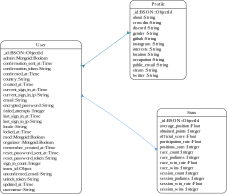
\includegraphics{datamodel1.png}
\end{center}

\begin{center}
	\includegraphics{datamodel2.png}
\end{center}


\begin{center}
	\includegraphics{datamodel3.png}
\end{center}

\begin{center}
	\includegraphics{datamodel4.png}
\end{center}

\section{Esquema de la Base de Datos}
A continuación, se describen los datos de la base de datos mediante archivos de definición de modelos de Ruby con mongoid:

\begin{listing}
  \begin{minted}[mathescape,
  	numbersep=5pt,
  	frame=single,
  	framesep=2mm]{ruby}
class Season
  include Mongoid::Document
  include Mongoid::Timestamps
  include Mongoid::MultiParameterAttributes
  
  store_in :database => 'rv_seasons'
  
  has_many :rankings
  has_many :cars
  has_many :tracks
  
  embeds_many :racer_result_entries
  
  accepts_nested_attributes_for :racer_result_entries
  
  field :name, :type => String
  field :start_date, :type => Date
  field :end_date, :type => Date
  field :current, :type => Boolean, :default => false
  
  validates_presence_of :name
  validates_presence_of :start_date
  validates_presence_of :current
  
  validates_uniqueness_of :name
end
  \end{minted}
  \caption[Esquema de Season]{Representación en código del modelo de Season de RVA.}
\end{listing}

\begin{listing}
\begin{minted}[mathescape,
	numbersep=5pt,
	gobble=2,
	frame=single,
	framesep=2mm]{ruby}
  class Ranking
    include Mongoid::Document
    include Mongoid::Timestamps
    
    store_in :database => 'rv_rankings'
    
    belongs_to :season
    has_many :sessions
    
    embeds_many :racer_result_entries
    
    accepts_nested_attributes_for :racer_result_entries
    
    field :number, :type => Integer
    
    validates_presence_of :number
	 end
\end{minted}
\caption[Esquema de Ranking]{Representación en código del modelo de Ranking de RVA.}
\end{listing}

\begin{listing}
  \begin{minted}[mathescape,
    numbersep=5pt,
    gobble=2,
    frame=single,
    framesep=2mm]{ruby}
    class Session
      include Mongoid::Document
      include SessionLogUploader::Attachment(:session_log)
      include Mongoid::Timestamps
      
      store_in :database => 'rv_sessions'
      
      belongs_to :ranking
      embeds_many :races
      embeds_many :racer_result_entries
      
      accepts_nested_attributes_for :racer_result_entries
      
      field :number, :type => Integer
      field :host, :type => String
      field :version, :type => String
      field :physics, :type => String
      field :protocol, :type => String
      field :pickups, :type => Boolean
      field :date, :type => Date
      field :teams, :type => Boolean
      field :category, :type => Integer
      field :session_log_data, :type => String
      
      validates_presence_of :number
      validates_presence_of :host
      validates_presence_of :version
      validates_presence_of :physics
      validates_presence_of :protocol
      validates_presence_of :date
      validates_presence_of :session_log
      validates_presence_of :teams
      validates_presence_of :category
    end
  \end{minted}
  \caption[Esquema de Session]{Representación en código del modelo de Session de RVA.}
\end{listing}

\begin{listing}
  \begin{minted}[mathescape,
    numbersep=5pt,
    gobble=2,
    frame=single,
    framesep=2mm]{ruby}
    class User
      include Mongoid::Document
      include Mongoid::Timestamps
      
      store_in :database => 'rv_users'
      
      USERNAME_REGEX = /\A([A-Z0-9_]{1,16}|[0-9a-f]{24})\z/
      
      validates :email, :presence => true, :uniqueness => true
      validates :username, :presence => true, 
        :uniqueness => true, 
        :length => { :minimum => 2, :maximum => 16 }
      validates_format_of :username, :with => USERNAME_REGEX
      
      belongs_to :team, :optional => true
      has_one :team
      
      embeds_one :profile
      embeds_one :stats
      accepts_nested_attributes_for(
        :profile,
        :update_only => true,
        :allow_destroy => false
      )
      accepts_nested_attributes_for(:stats,
        :update_only => true,
        :allow_destroy => false
      )
      
      before_create :create_profile
      before_create :create_stats
      
      field :admin, :type => Boolean, :default => false
      field :mod, :type => Boolean, :default => false
      field :organizer, :type => Boolean, :default => false
      field :locale, :type => String, :default => 'en_us'
      field :country, :type => String
    end
  \end{minted}
  \caption[Esquema de Session]{Representación en código del modelo de Session de RVA.}
\end{listing}

\begin{listing}
  \begin{minted}[mathescape,
    numbersep=5pt,
    gobble=2,
    frame=single,
    framesep=2mm]{ruby}
    class Race
      include Mongoid::Document
      include Mongoid::Attributes::Dynamic
      
      embedded_in :session
      
      embeds_many :racer_entries
      
      field :track_name, :type => String
      field :laps, :type => Integer
      field :racers_count, :type => Integer
      
      validates_presence_of :track_name
      validates_presence_of :laps
      validates_presence_of :racers_count
    end
  \end{minted}
  \caption[Esquema de Profile]{Representación en código del modelo Profile.}
\end{listing}

\begin{listing}
  \begin{minted}[mathescape,
    numbersep=5pt,
    gobble=2,
    frame=single,
    framesep=2mm]{ruby}
    class RacerEntry
      include Mongoid::Document
      include Mongoid::Attributes::Dynamic
      
      embedded_in :race
      
      field :car_name, :type => String
      field :position, :type => Integer
      field :username, :type => String
      field :time, :type => String
      field :best_lap, :type => String
      field :finished, :type => Mongoid::Boolean
      field :cheating, :type => Mongoid::Boolean
      
      validates_presence_of :car_name
      validates_presence_of :position
      validates_presence_of :username
      validates_presence_of :time
      validates_presence_of :best_lap
      validates_presence_of :finished
      validates_presence_of :cheating
    end
  \end{minted}
  \caption[Esquema de Profile]{Representación en código del modelo Profile.}
\end{listing}

\begin{listing}
  \begin{minted}[mathescape,
    numbersep=5pt,
    gobble=2,
    frame=single,
    framesep=2mm]{ruby}
    class Profile
      include Mongoid::Document
      
      embedded_in :user
      
      field :about, :type => String
      field :gender, :type => String
      field :public_email, :type => String
      field :location, :type => String
      field :discord, :type => String
      field :github, :type => String
      field :instagram, :type => String
      field :crowdin, :type => String
      field :steam, :type => String
      field :twitter, :type => String
      field :occupation, :type => String
      field :interests, :type => String
    end
  \end{minted}
  \caption[Esquema de Profile]{Representación en código del modelo Profile.}
\end{listing}

\begin{listing}
  \begin{minted}[mathescape,
    numbersep=5pt,
    gobble=2,
    frame=single,
    framesep=2mm]{ruby}
    class Stats
      include Mongoid::Document
      
      embedded_in :user
      
      field :race_wins, :type => Integer
      field :race_win_rate, :type => Float
      field :race_podiums, :type => Integer
      field :race_count, :type => Integer
      field :positions_sum, :type => Integer
      field :session_wins, :type => Integer
      field :session_win_rate, :type => Float
      field :session_podiums, :type => Integer
      field :session_count, :type => Integer
      field :average_position, :type => Float
      field :participation_rate, :type => Float
      field :official_score, :type => Float
      field :obtained_points, :type => Integer
    end
  \end{minted}
  \caption[Esquema de Stats]{Representación en código del modelo Stats.}
\end{listing}

\begin{listing}
  \begin{minted}[mathescape,
    numbersep=5pt,
    gobble=2,
    frame=single,
    framesep=2mm]{ruby}
    class Car
      include Mongoid::Document
      include Mongoid::Timestamps
      
      store_in :database => 'rv_cars'
      
      belongs_to :season
      
      field :name, :type => String
      field :speed, :type => Float
      field :accel, :type => Float
      field :weight, :type => Float
      field :multiplier, :type => Float
      field :folder_name, :type => String
      field :category, :type => Integer
      field :stock, :type => Boolean, :default => false
      
      validates_presence_of :name
      validates_presence_of :speed
      validates_presence_of :accel
      validates_presence_of :weight
      validates_presence_of :multiplier
      validates_presence_of :folder_name
      validates_presence_of :category
      validates_presence_of :stock
    end
  \end{minted}
  \caption[Esquema de Car]{Representación en código del modelo Car.}
\end{listing}

\begin{listing}
  \begin{minted}[mathescape,
    numbersep=5pt,
    gobble=2,
    frame=single,
    framesep=2mm]{ruby}
    class Track
      include Mongoid::Document
      include Mongoid::Timestamps
      
      store_in :database => 'rv_tracks'
      
      belongs_to :season
      
      field :name, :type => String
      field :short_name, :type => String
      field :difficulty, :type => Integer
      field :length, :type => Integer
      field :folder_name, :type => String
      field :stock, :type => Boolean, :default => false
      
      validates_presence_of :name
      validates_presence_of :short_name
      validates_presence_of :difficulty
      validates_presence_of :length
      validates_presence_of :folder_name
      validates_presence_of :stock
    end
  \end{minted}
  \caption[Esquema de Track]{Representación en código del modelo Track.}
\end{listing}

\begin{listing}
  \begin{minted}[mathescape,
    numbersep=5pt,
    gobble=2,
    frame=single,
    framesep=2mm]{ruby}
    class RacerResultEntry
      include Mongoid::Document
      
      embedded_in :season
      embedded_in :ranking
      embedded_in :session
      
      field :username, :type => String
      field :country, :type => String
      field :session_count, :type => Integer
      field :race_count, :type => Integer
      field :positions_sum, :type => Integer
      field :average_position, :type => Float
      field :obtained_points, :type => Integer
      field :official_score, :type => Float
      field :participation_multiplier, :type => Float
      field :team, :type => String
      
      validates_presence_of :username
      validates_presence_of :country
    end
  \end{minted}
  \caption[Esquema de Track]{Representación en código del modelo Track.}
\end{listing}

\clearpage

\section{Diseño de Interfaz}

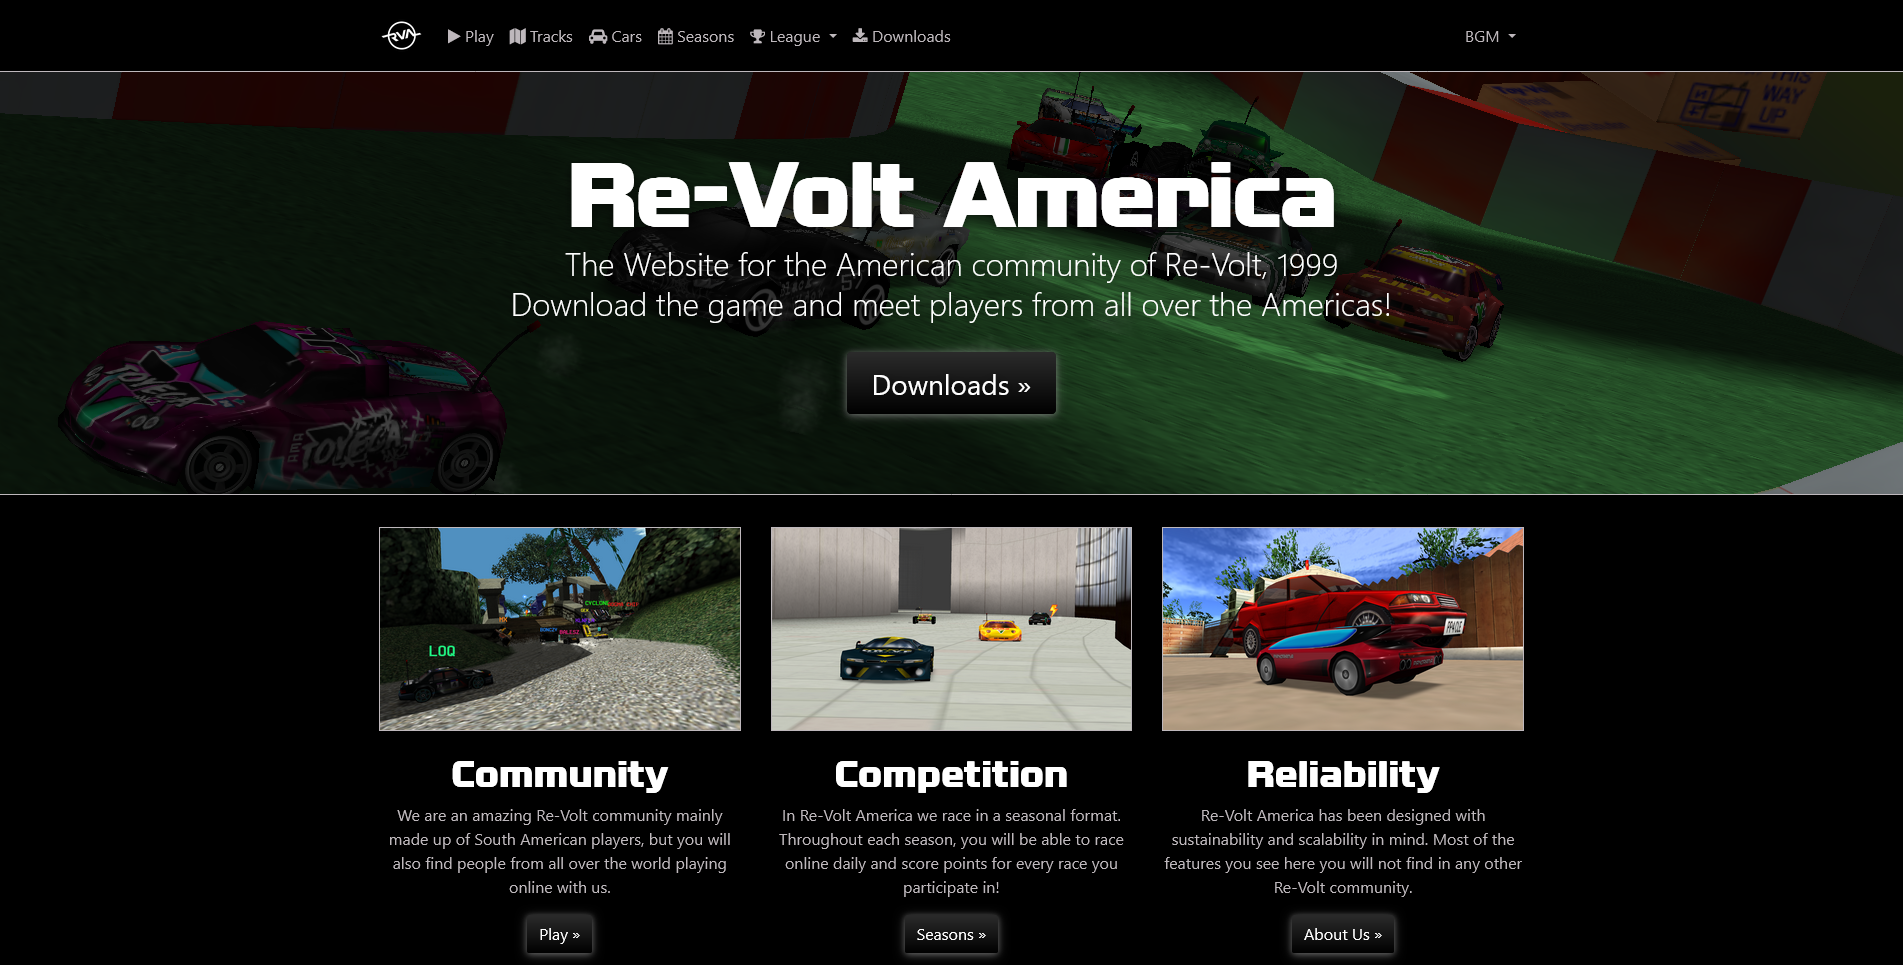
\includegraphics[width=15cm, height=8cm]{img/landing.png} \\

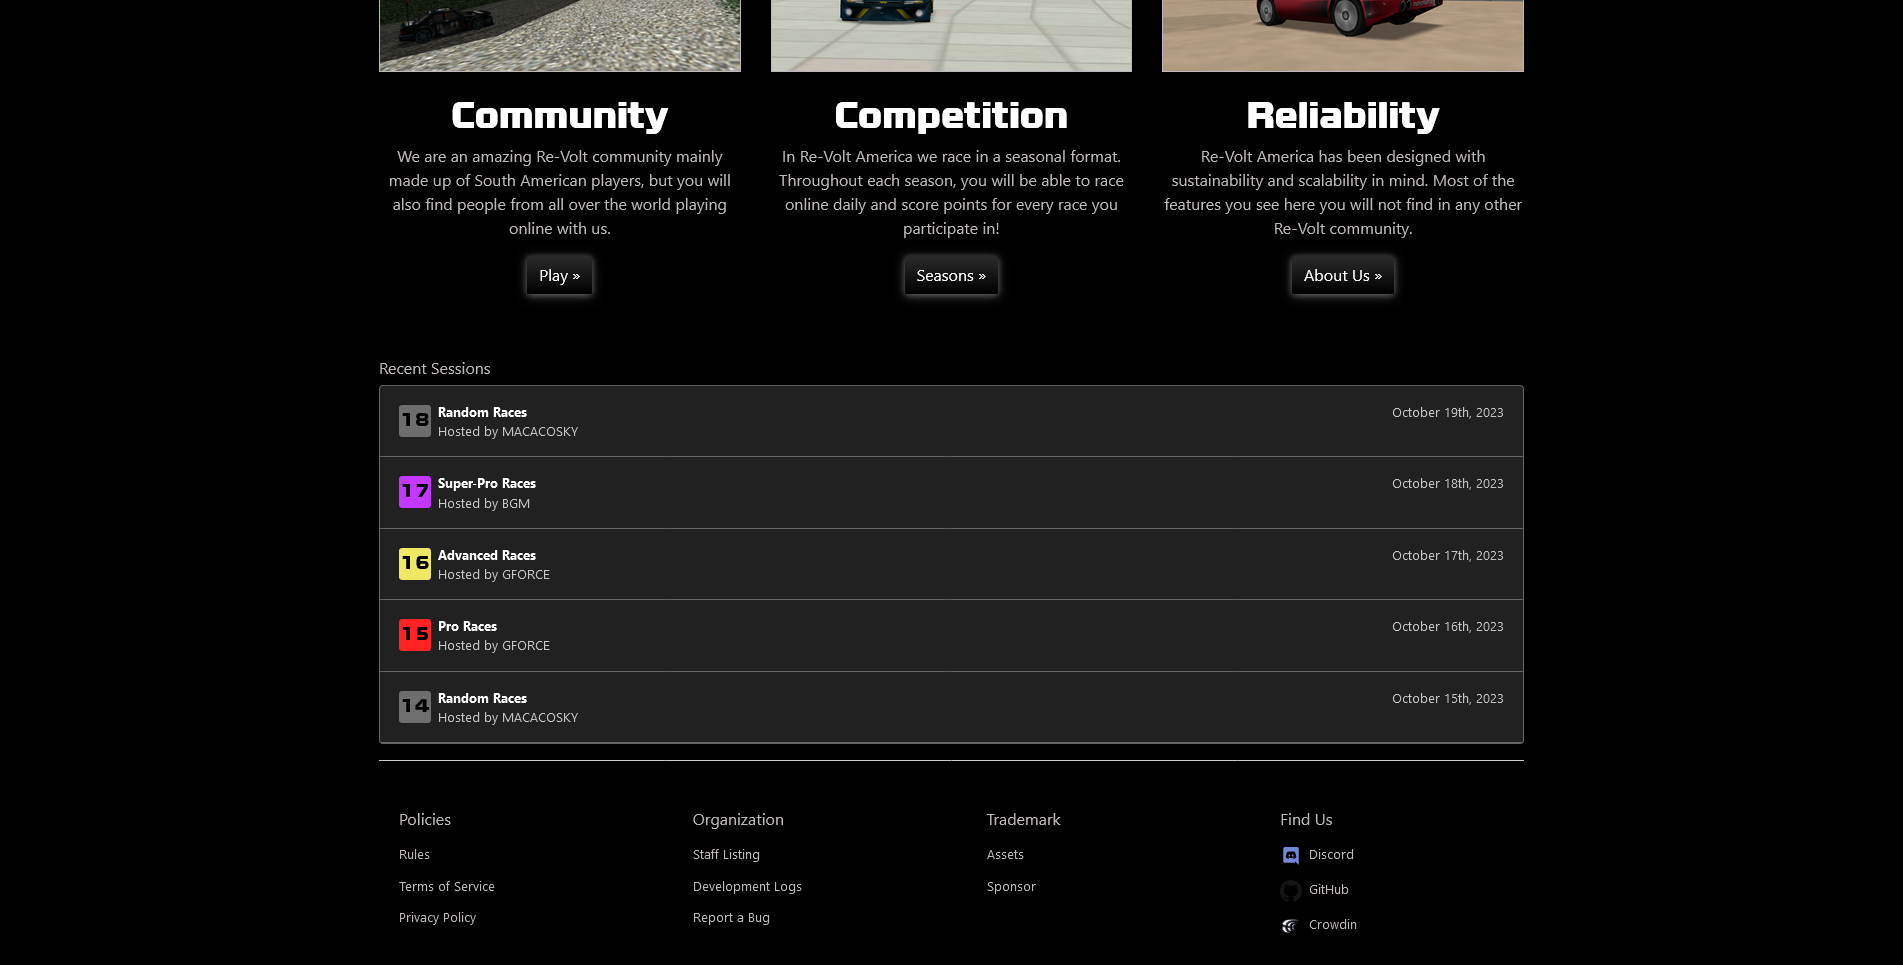
\includegraphics[width=15cm, height=8cm]{img/landing2.png} \\

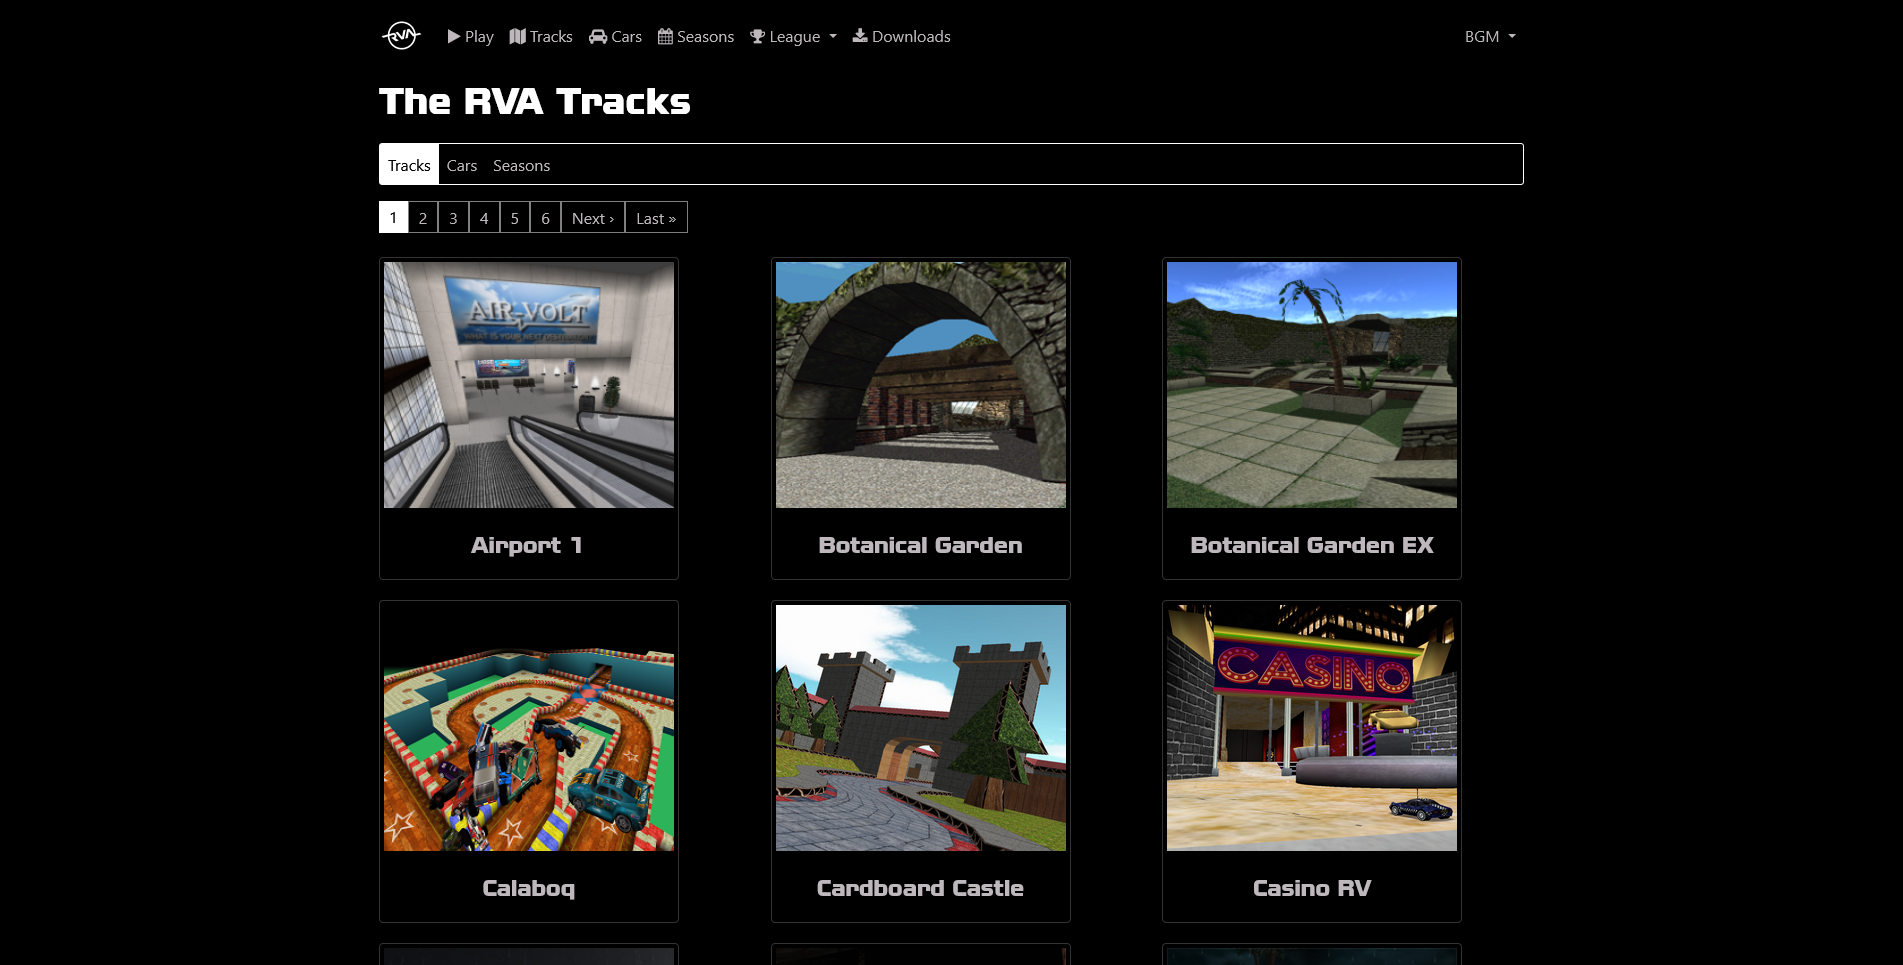
\includegraphics[width=15cm, height=8cm]{img/tracks.png} \\

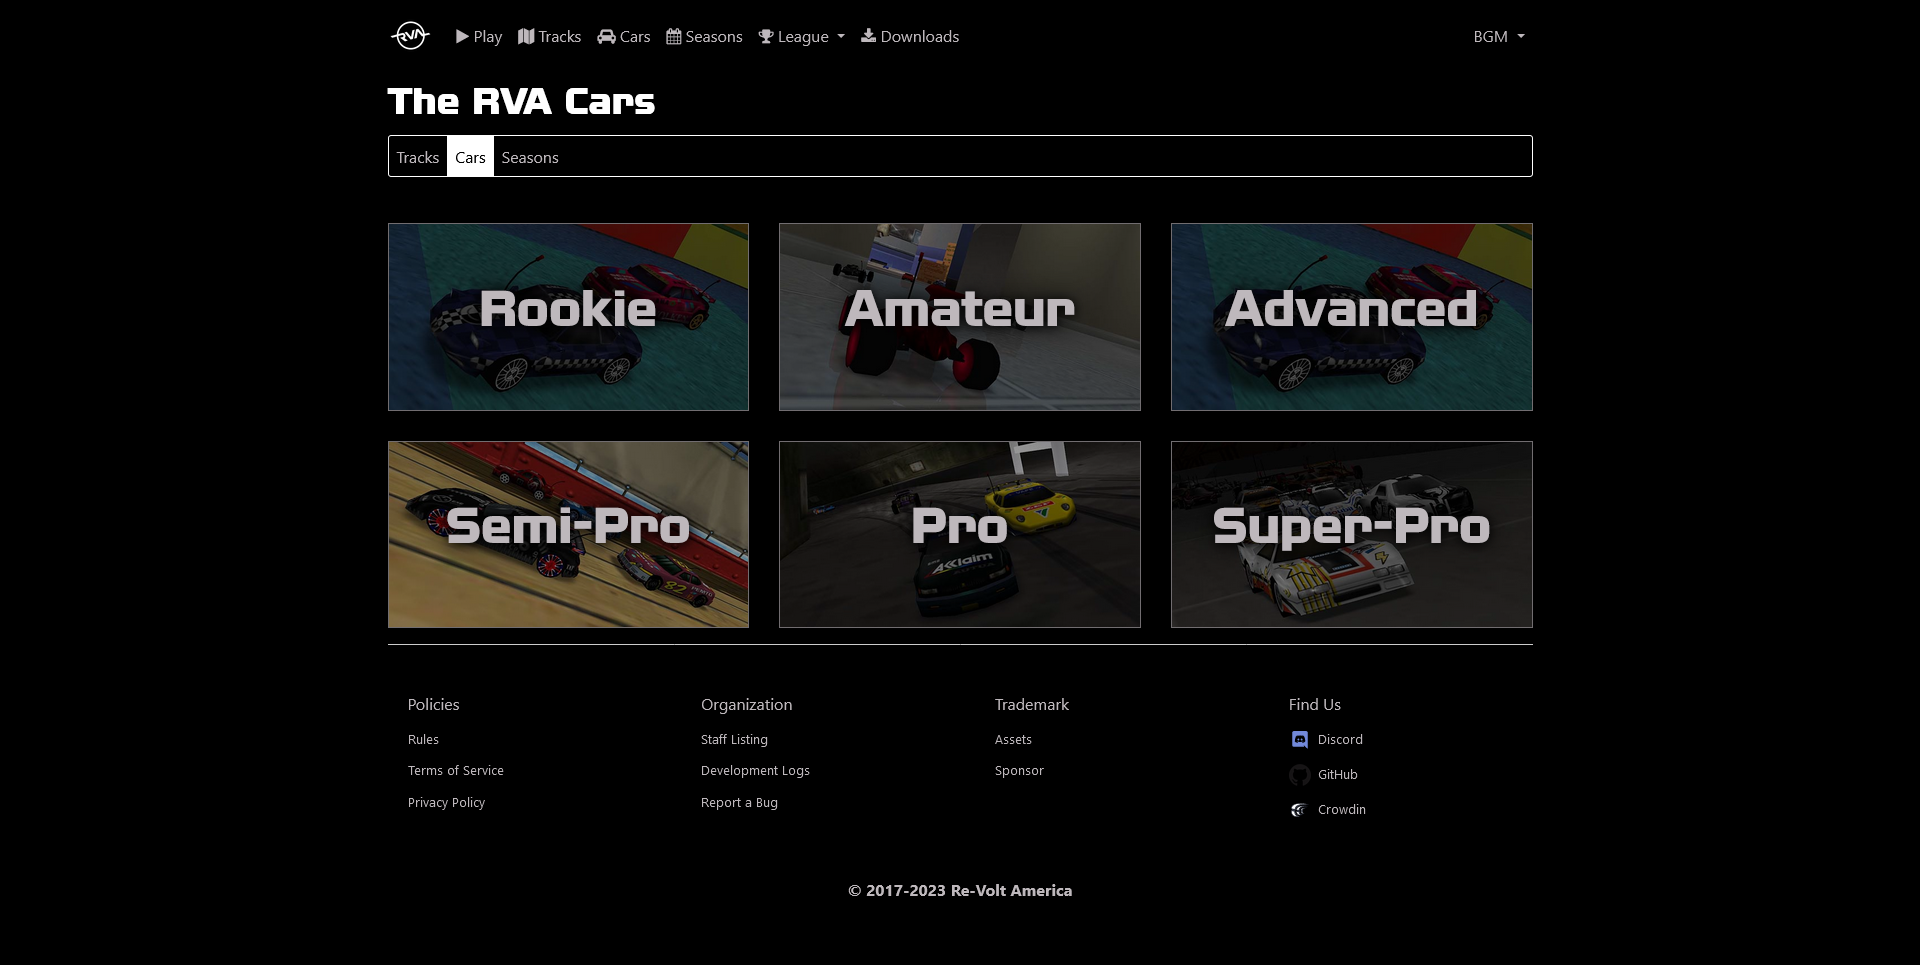
\includegraphics[width=15cm, height=8cm]{img/cars.png} \\

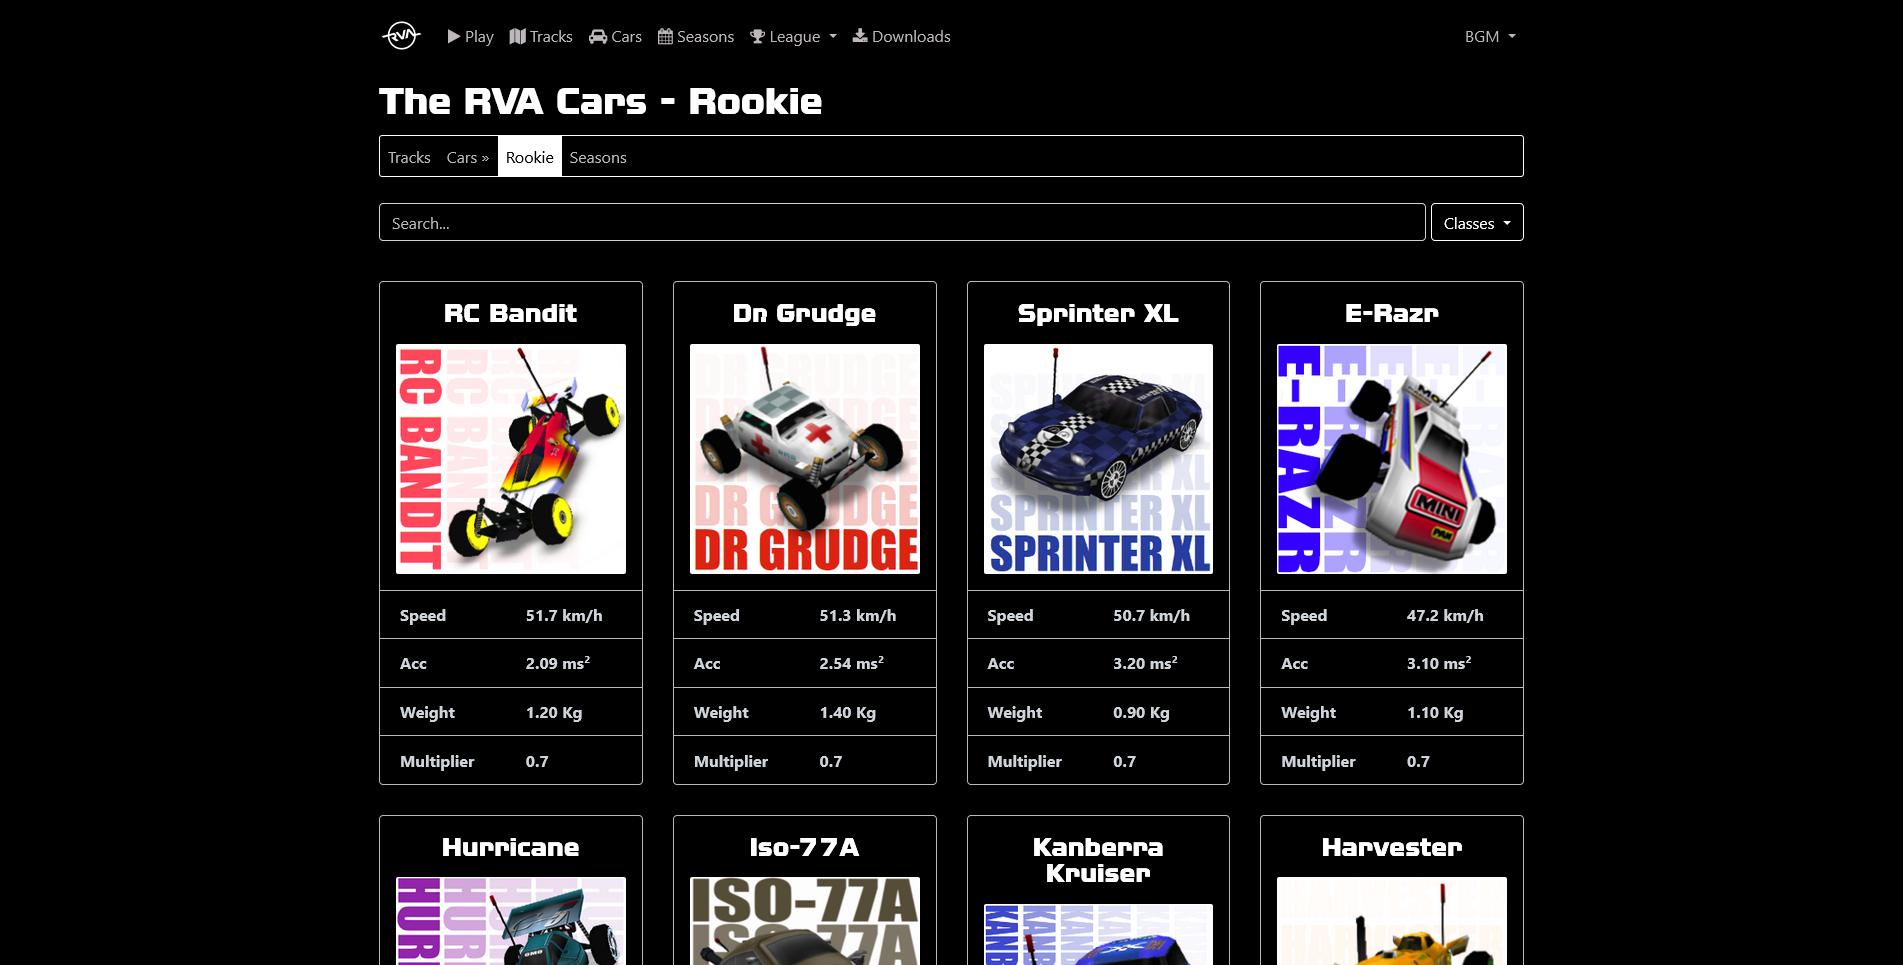
\includegraphics[width=15cm, height=8cm]{img/cars2.png} \\

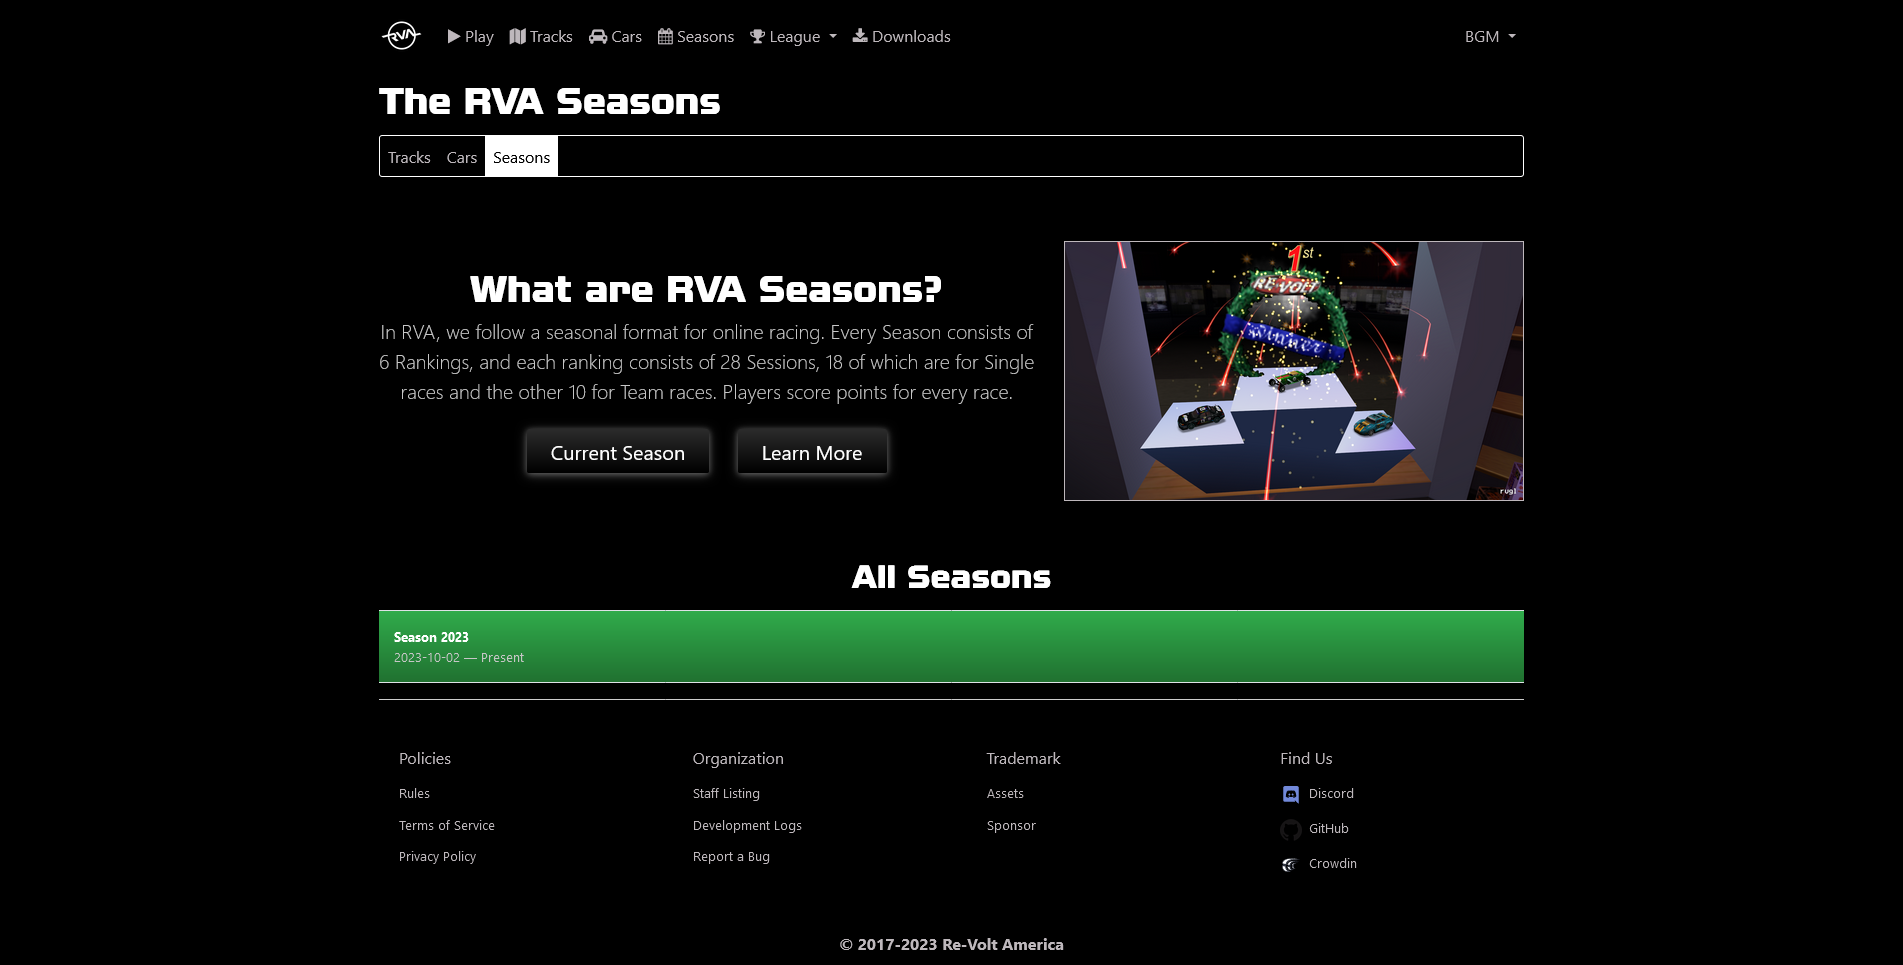
\includegraphics[width=15cm, height=8cm]{img/seasons.png} \\

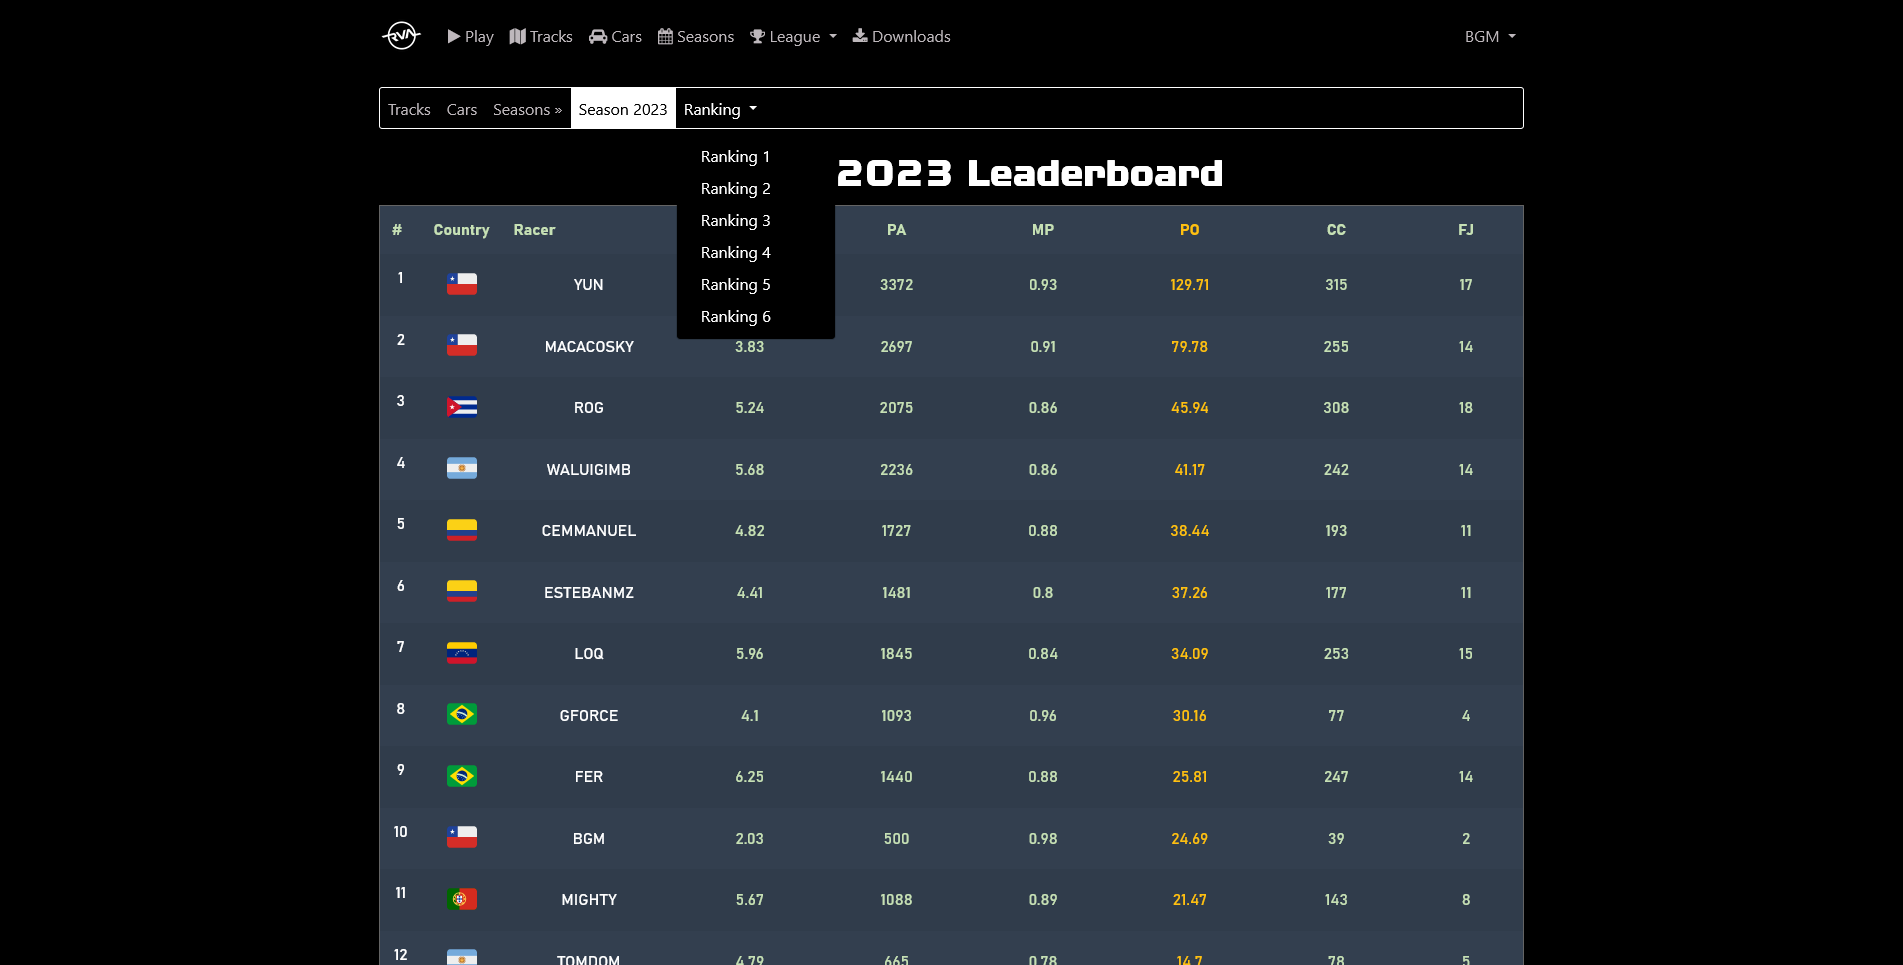
\includegraphics[width=15cm, height=8cm]{img/season.png} \\

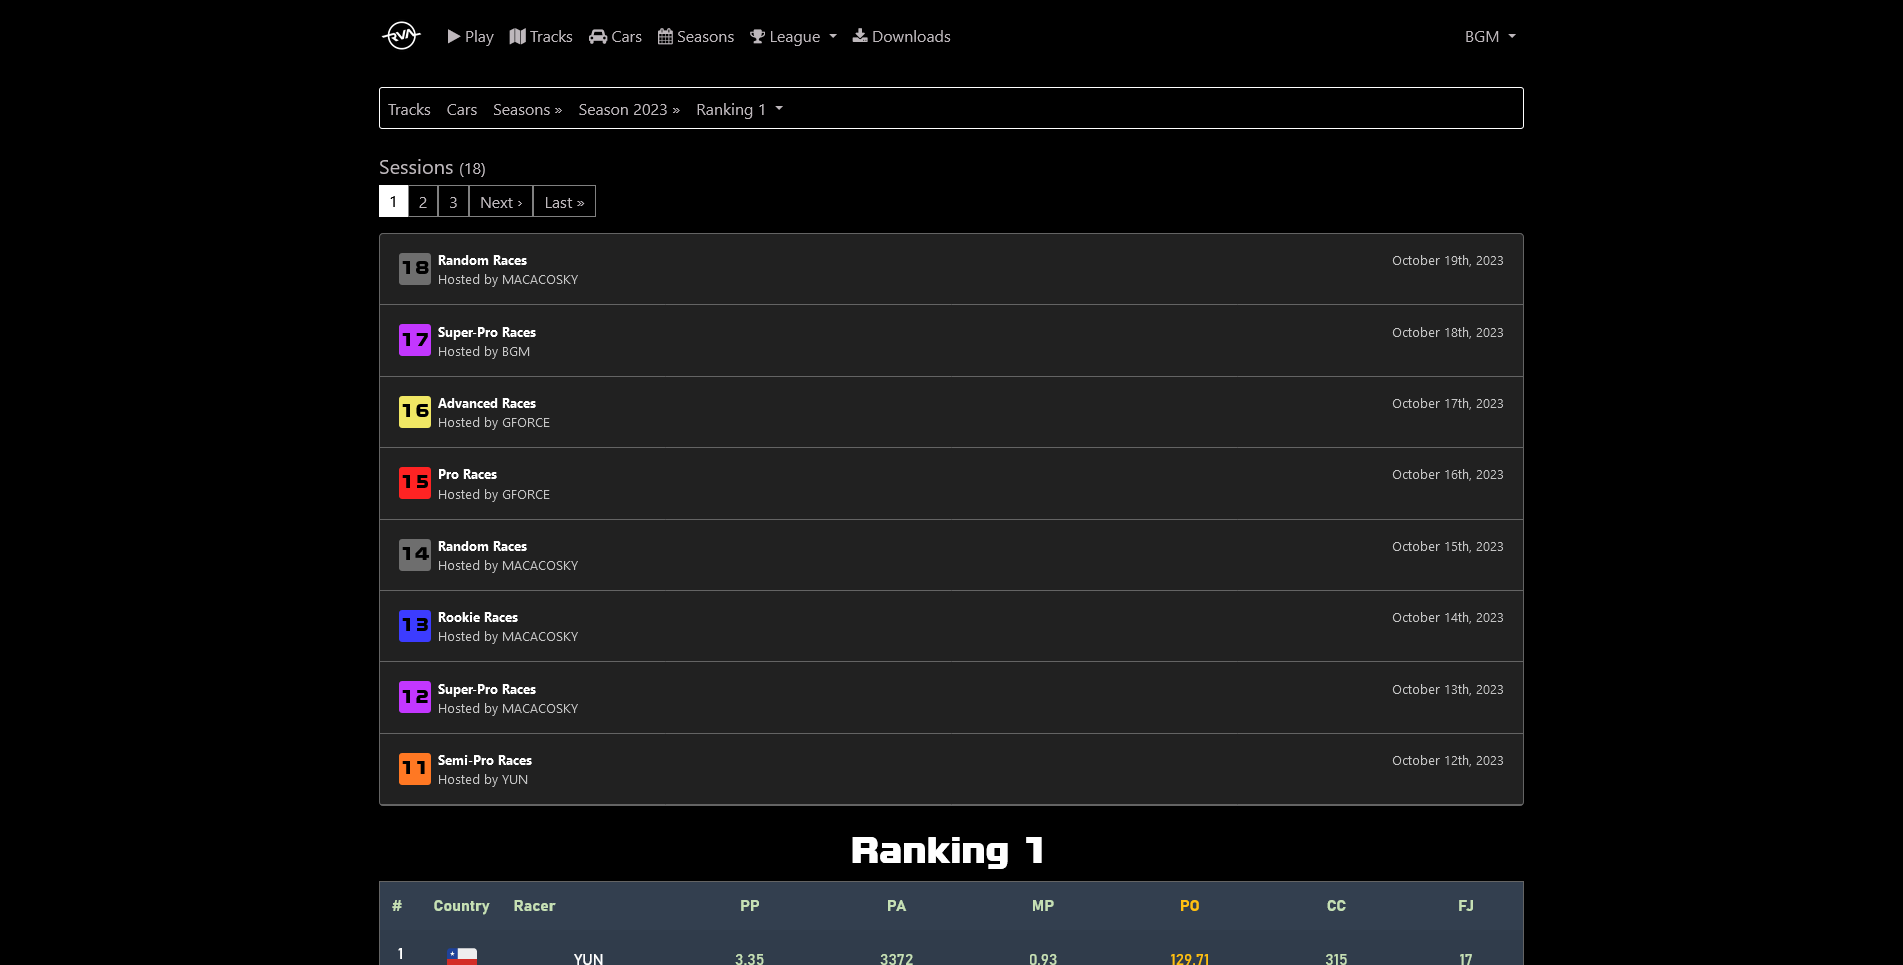
\includegraphics[width=15cm, height=8cm]{img/ranking.png} \\

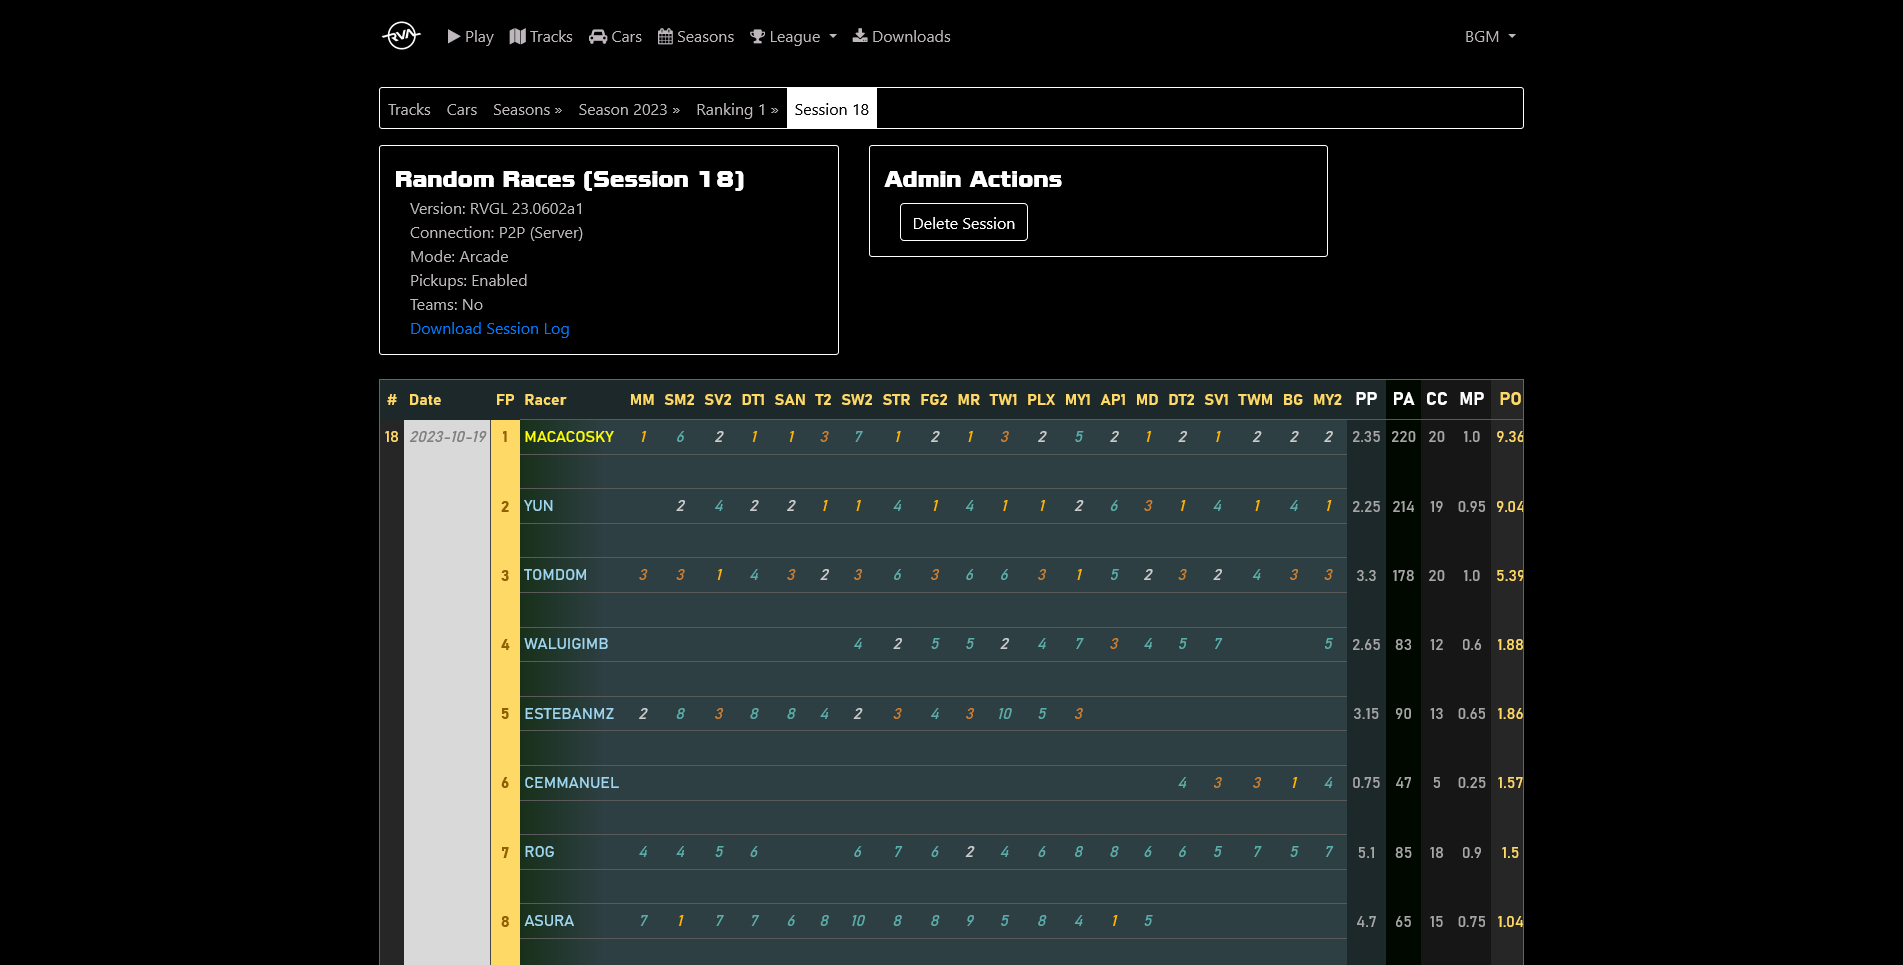
\includegraphics[width=15cm, height=8cm]{img/session.png} \\

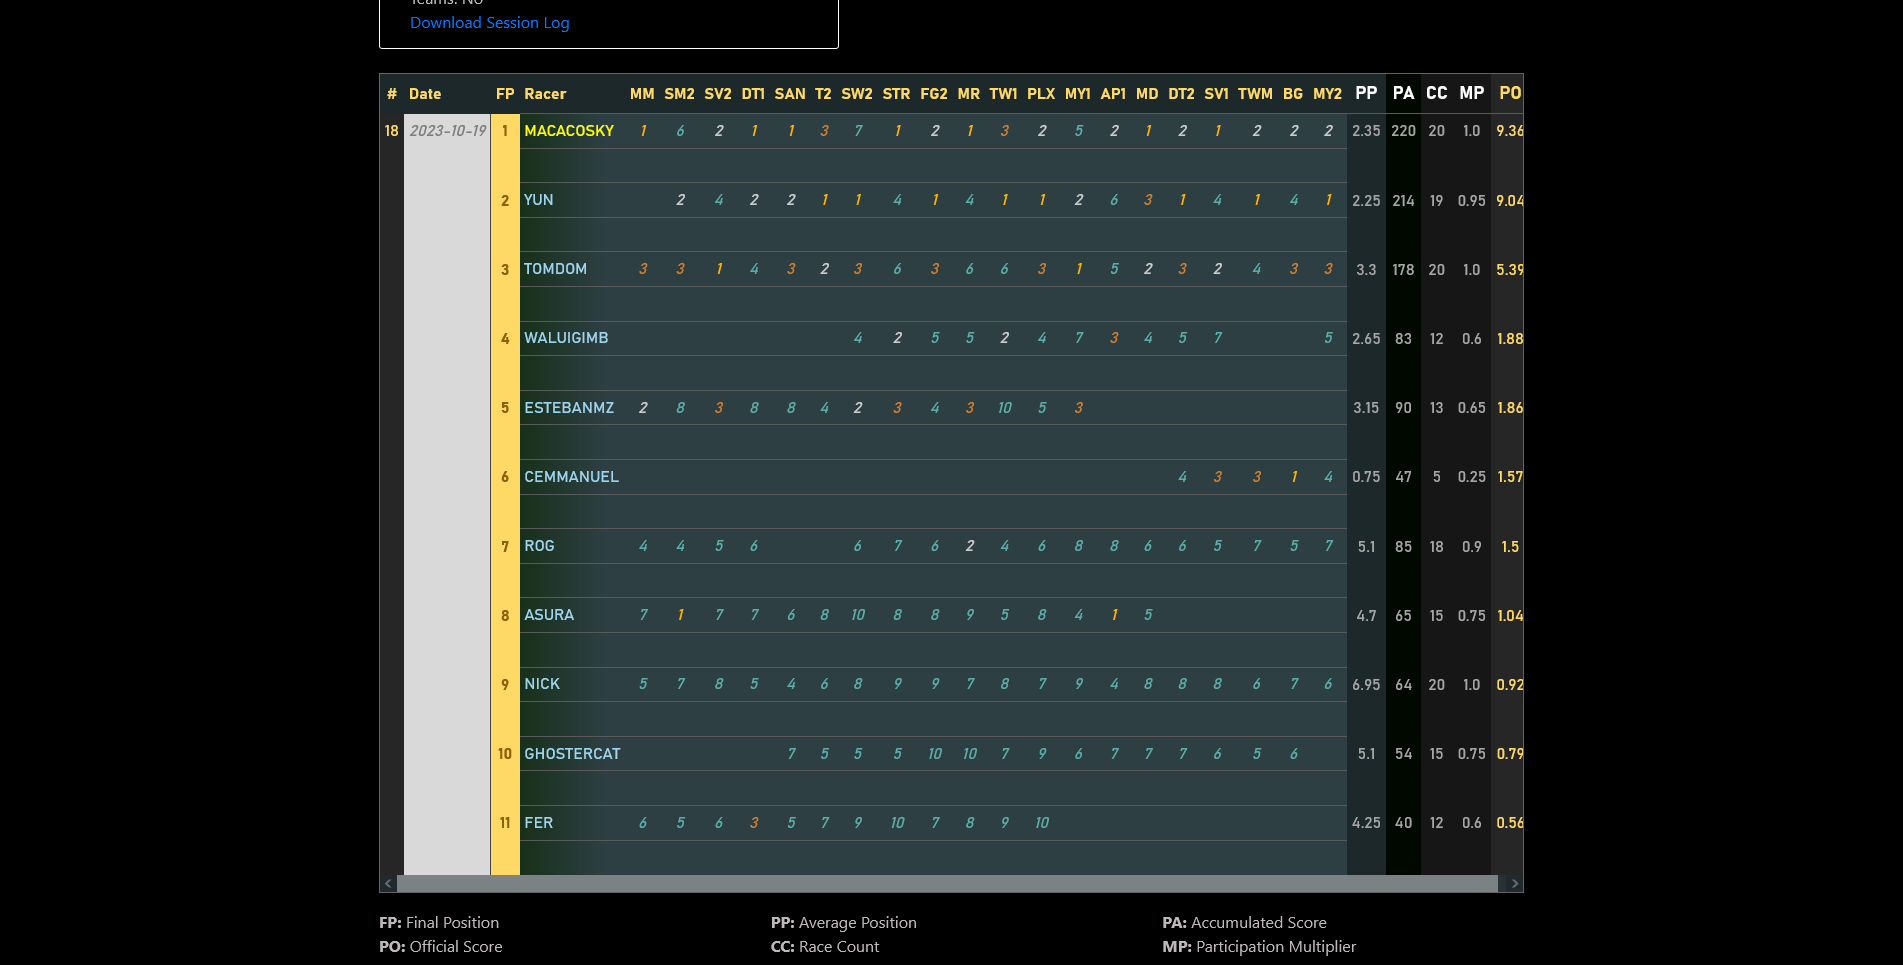
\includegraphics[width=15cm, height=8cm]{img/session2.png} \\

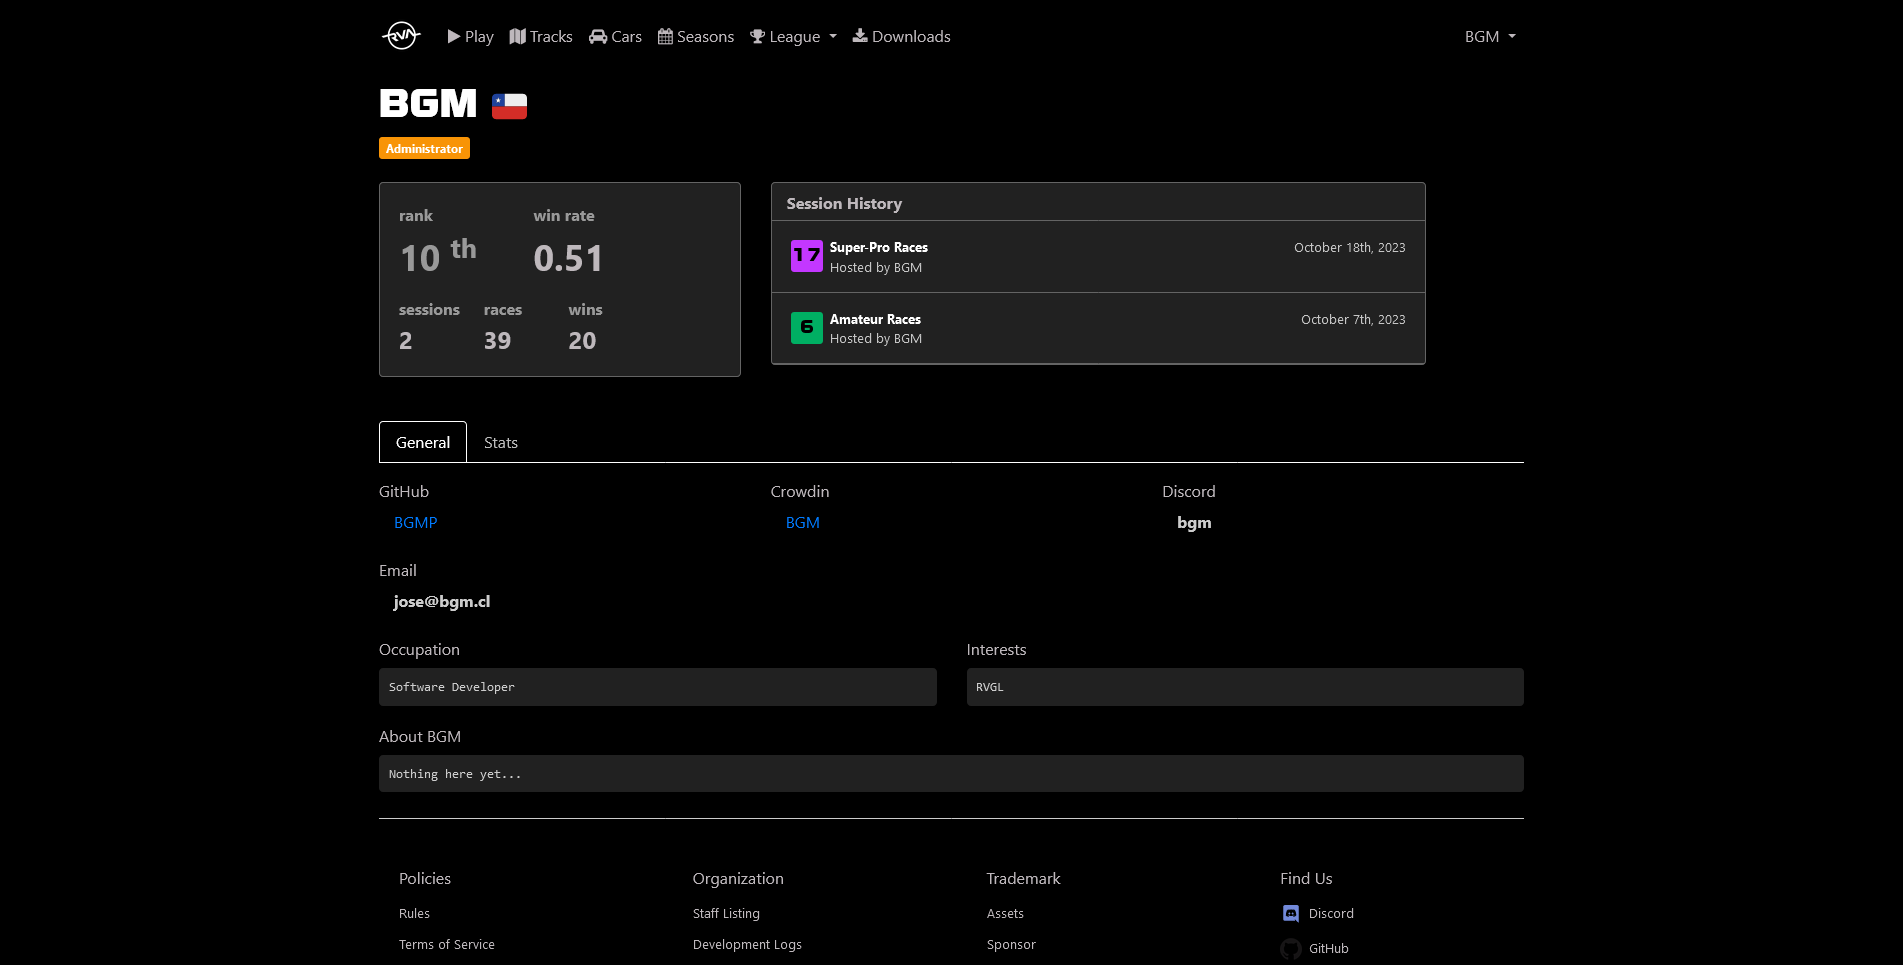
\includegraphics[width=15cm, height=8cm]{img/profile.png} \\

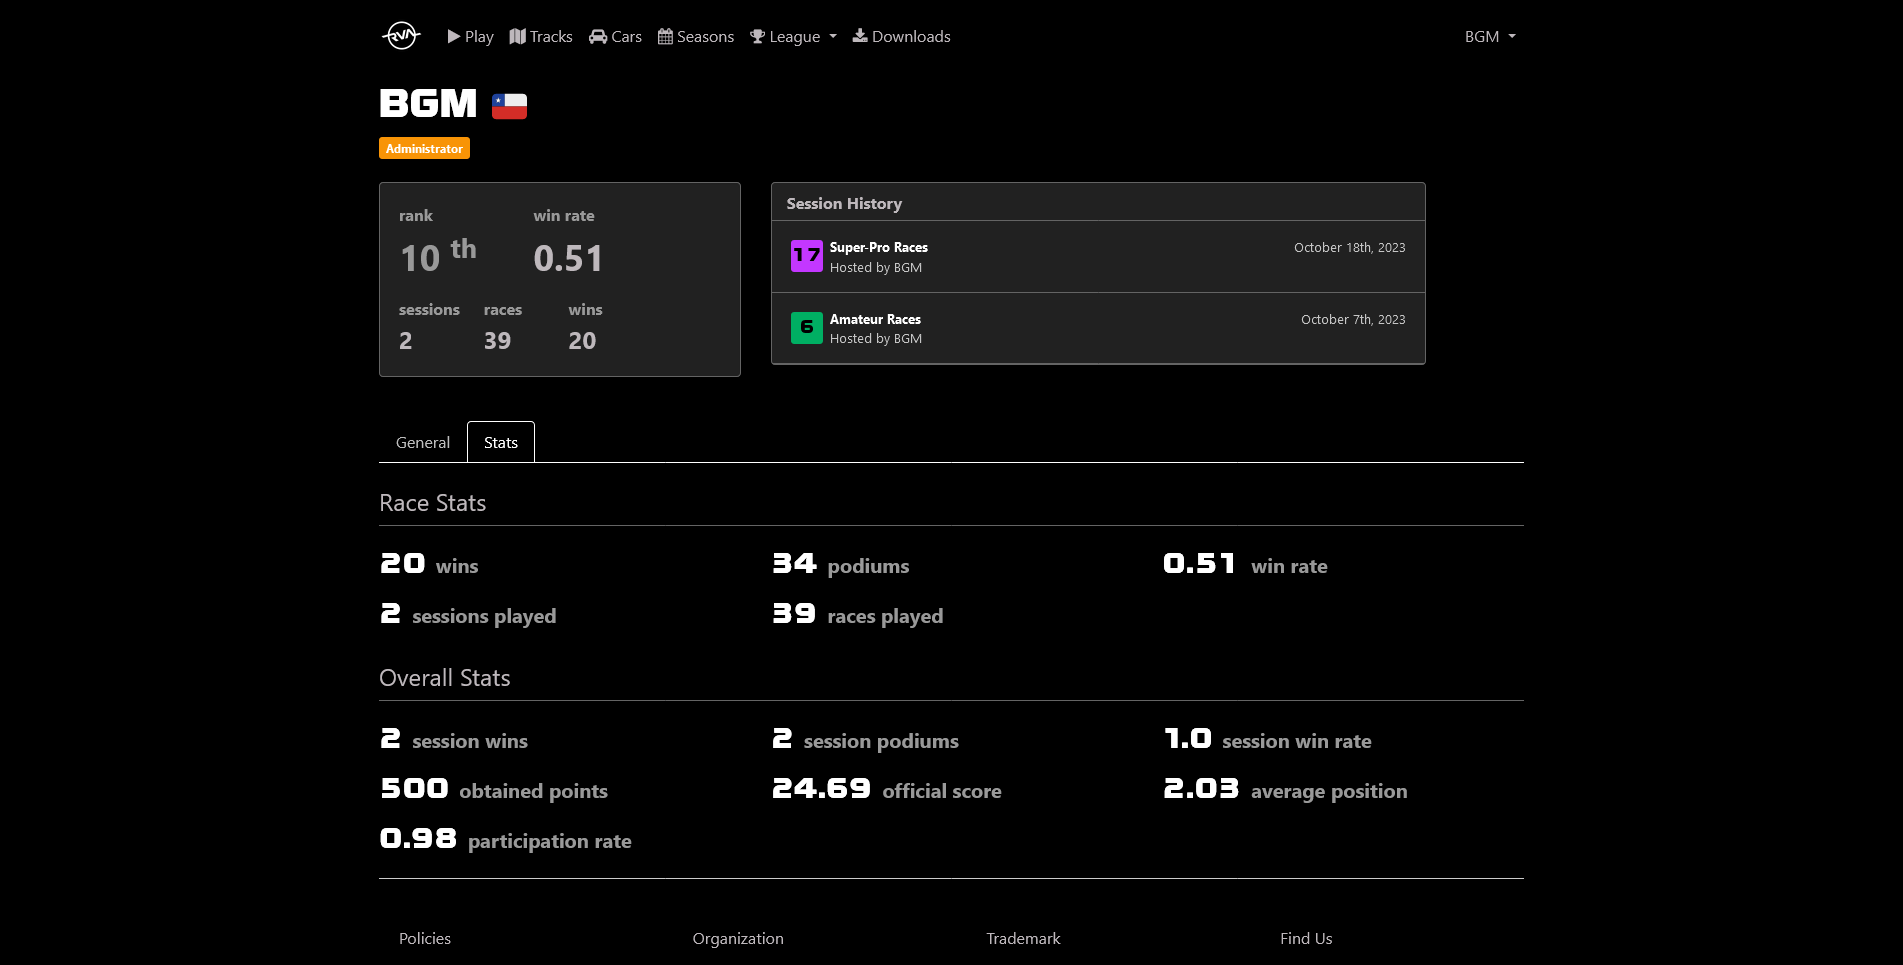
\includegraphics[width=15cm, height=8cm]{img/profile1.png} \\

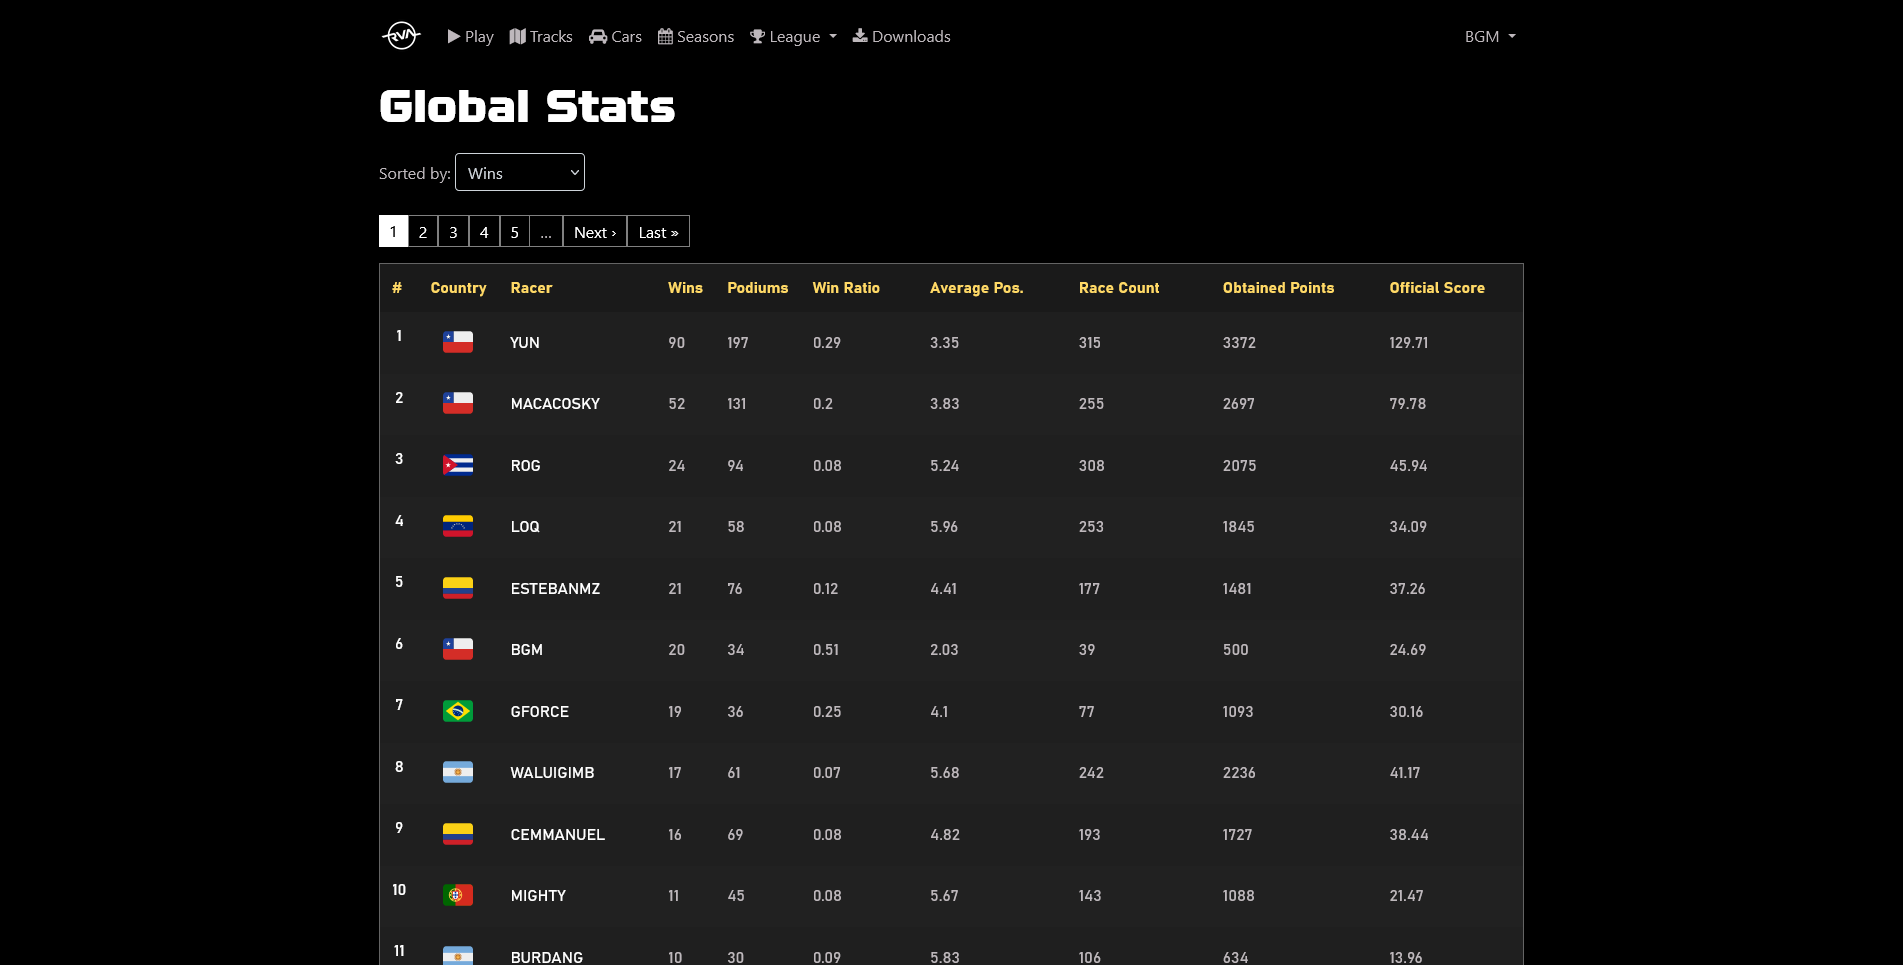
\includegraphics[width=15cm, height=8cm]{img/stats.png} \\

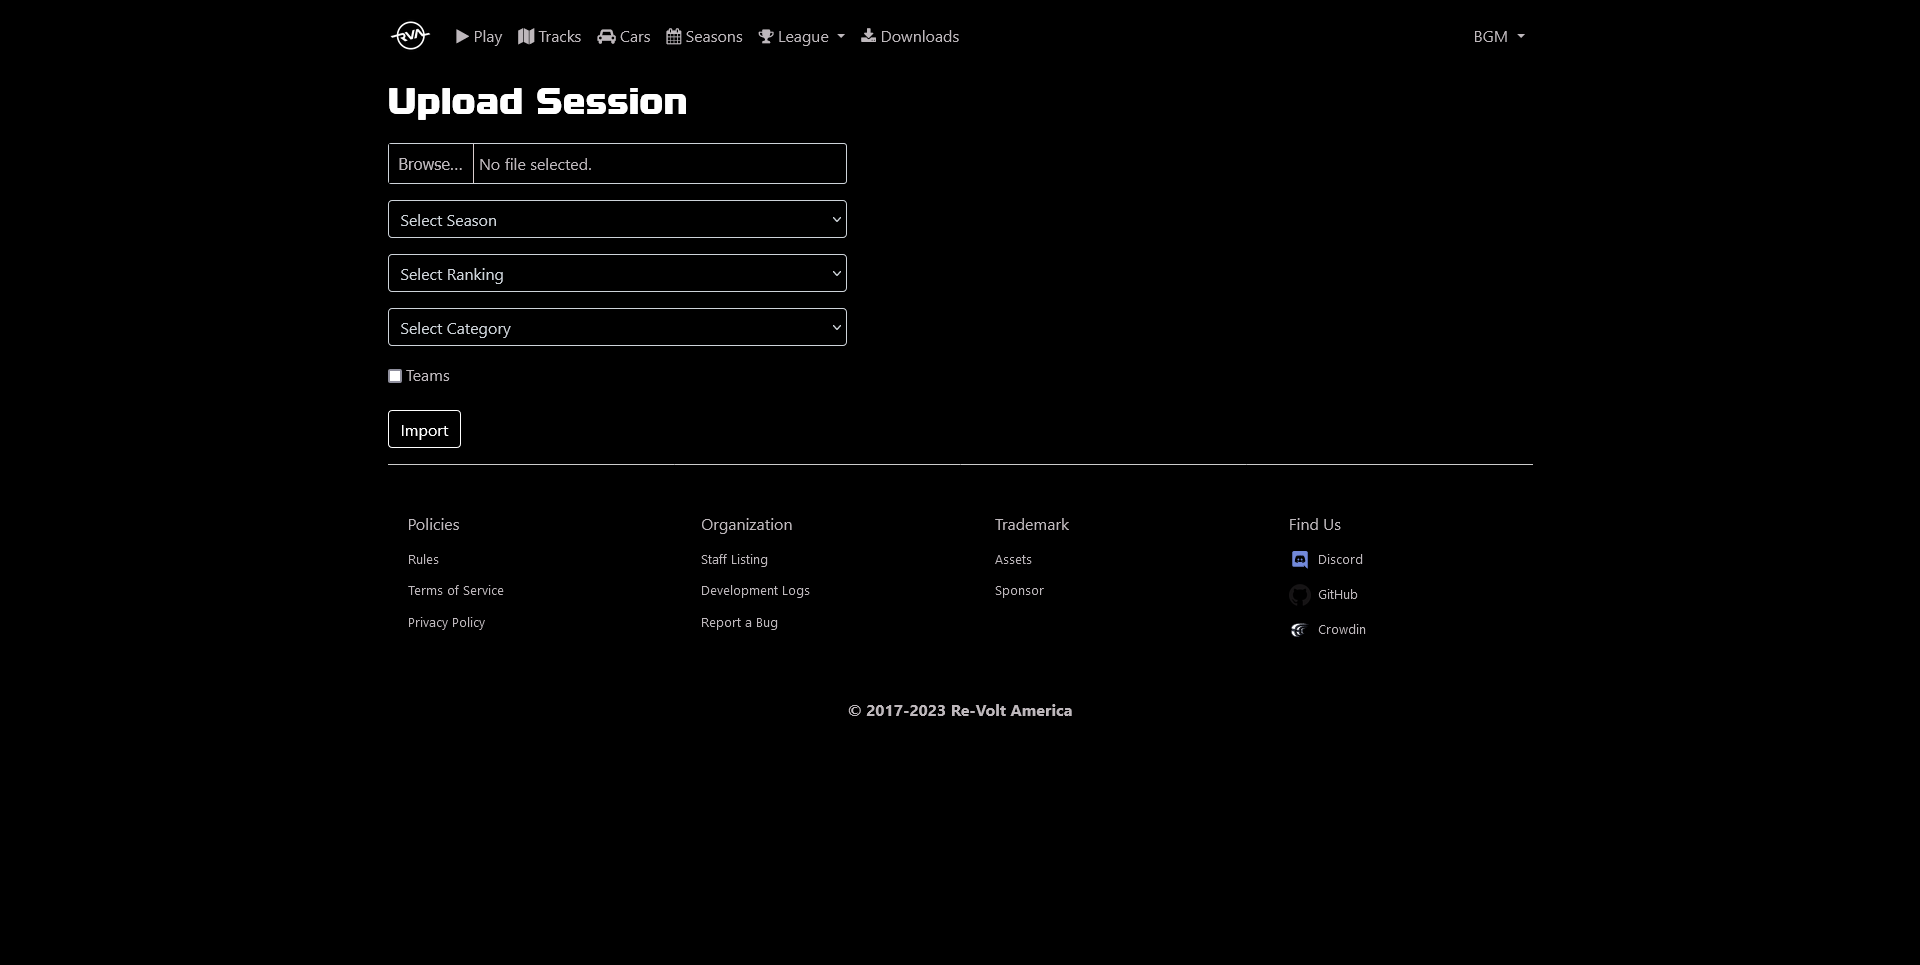
\includegraphics[width=15cm, height=8cm]{img/upload.png}

\subsection{Fuentes}

\begin{center}
  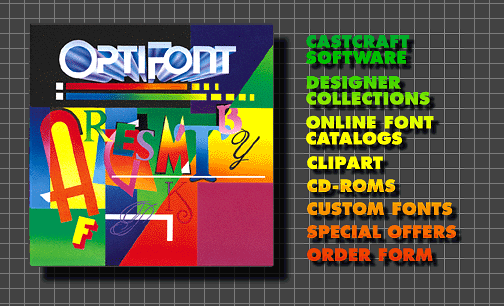
\includegraphics{optifont.png}
\end{center}

\subsection{Paleta de Colores}






















\section{Diseño de Arquitectura}
El proyecto, en su estado actual, hace uso de un servidor propio, el cual contiene los servicios web, bases de datos y caché. Todo en una sola máquina. Independientemente de donde se termine alojanda, la aplicación web estará disponible en ''https://rva.lat/''.

Además de esto, la planificación contempla dos servicios externos, que actualmente son proveídos por GitHub pages, los cuales sirven como repositorios de almacenamiento de datos masivos. Dichos repositorios se encargan actualmente de servir información y assets como las imágenes de las pistas y autos que la web ofrece a los usuarios:

\begin{itemize}
	\item https://tracks.rva.lat/: Repositorio de pistas de RVA.
	\item https://cars.rva.lat/: Repositorio de autos de RVA.
\end{itemize}

A continuación, se muestra un diagrama que ilustra todo el proceso de interacción entre servicios y usuarios:

Tal como se puede apreciar en la ilustración anterior, la arquitectura que da soporte a la aplicación web de RVA se concentra en un servidor, con dos almacenes de datos. Podemos ver que los usuarios juegan la sesión, el host de la sesión sube el Session Log a la web, y los usuarios pueden visitar la misma web para revisar los resultados

\section{Estructura del código}
El proyecto, al ser una aplicación hecha en el framework de Ruby on Rails, sigue patrón de MVC (Model View Controller), o modelo, vista, controlador. El árbol de directorio se ve de la siguiente manera:

% IMAGEN

Todas las bases de datos dentro de MongoDB están prefijadas utilizando el término “rv”. Por ejemplo, la base de datos que almacena las colecciones de autos se llama “rv\_cars”, la de los usuarios “rv\_users”, etc.

\subsection{Backend}

\begin{center}
  \begin{tabular}{ | l | p{12.5cm} |}
    \hline
    \multicolumn{1}{|c|}{\textbf{Directorio}} & \multicolumn{1}{|c|}{\textbf{Detalle}} \\
    \hline
    
    {\textbf{controllers}} & Contiene todos los controladores de Rails, los cuales manejan todas las peticiones web del usuario. \\ \hline
    
    {\textbf{helpers}} & Contiene todas las clases utilitarias, las cuales pueden ser utilizadas para asistir a las clases de modelos, vistas y controladores. \\ \hline
    
    {\textbf{javascript}} & Todo el código de JavaScript utilizado por la aplicación a nivel web se almacena en este directorio.\\ \hline
    
    {\textbf{models}} & Contiene todas las clases que modelan y envuelven los datos almacenados en la base de datos de la aplicación. \\ \hline
    
    {\textbf{services}} & Contiene todas las clases de servicio de la aplicación. Las clases de servicio son aquellos procesos complejos compuestos de mucho código, los cuales se abstraen en servicios para no polucionar los controladores que los requieren. \\ \hline
    
    {\textbf{uploaders}} & Contiene todas las clases relacionadas con la subida de archivos. \\ \hline
    
    {\textbf{config}} & Contiene toda la configuración de la aplicación, como las rutas, inicializadores de librerías, configuración de despliegue, declaración de los entornos de Rails (development, production), configuración de la base de datos y archivos de idioma para la localización del proyecto.\\ \hline
  \end{tabular}
\end{center}

\subsection{Frontend}

\begin{center}
  \begin{tabular}{ | l | p{12.5cm} |}
    \hline
    \multicolumn{1}{|c|}{\textbf{Directorio}} & \multicolumn{1}{|c|}{\textbf{Detalle}} \\
    \hline
    
    {\textbf{views}} & Contiene todas las vistas de la aplicación. Todo lo que el usuario ve en la aplicación web tiene su archivo de vista que lo representa. \\ \hline
    
    {\textbf{assets}} & Todas las imágenes, hojas de estilo y demás artefactos requeridos por la aplicación para su correcto funcionamiento y diseño. \\ \hline
    
    {\textbf{public}} & Todos los archivos estáticos servidos por la página pueden encontrarse aquí. Cosas como las páginas de error (404, 422, 500, etc.), estilos compilados, entre otros.\\ \hline
  \end{tabular}
\end{center}




